\documentclass[a4paper, 12pt]{article}

\usepackage[top=2cm, bottom=2cm, left=2.5cm, right=2.5cm]{geometry}
\usepackage[utf8]{inputenc}
\usepackage{array}
\usepackage{graphicx}
\usepackage{listings}
\usepackage{caption}
\usepackage{float}
\usepackage[labelfont=bf]{caption}

\captionsetup[lstlistings]{position=bottom}
\graphicspath{{img/}}

\begin{document}
\lstset{language=SQL}
\begin{flushleft}
\includegraphics{logo}\\
\textbf{UNIVERSIDADE TECNOLÓGICA FEDERAL DO PARANÁ | UTFPR} \\
\textbf{ALUNO:} Ricardo Medeiros da Costa Junior   \textbf{RA:} a1598996 \\
\textbf{DISCIPLINA:} Banco de Dados para Biologia \\
\textbf{ATIVIDADE:} Sistema de Recomendações | Tarefa 2 

\section{Persistência dos dados}
Foram persistidos todos os nós e relações no banco de dados, exatamente como foi orientado no documento da atividade, utilizando a linguagem \emph{Cypher}. Após realizado todas inserções, o banco de dados completo é semelhante ao da Figura 1. 

\begin{figure}[H]
  \centering
  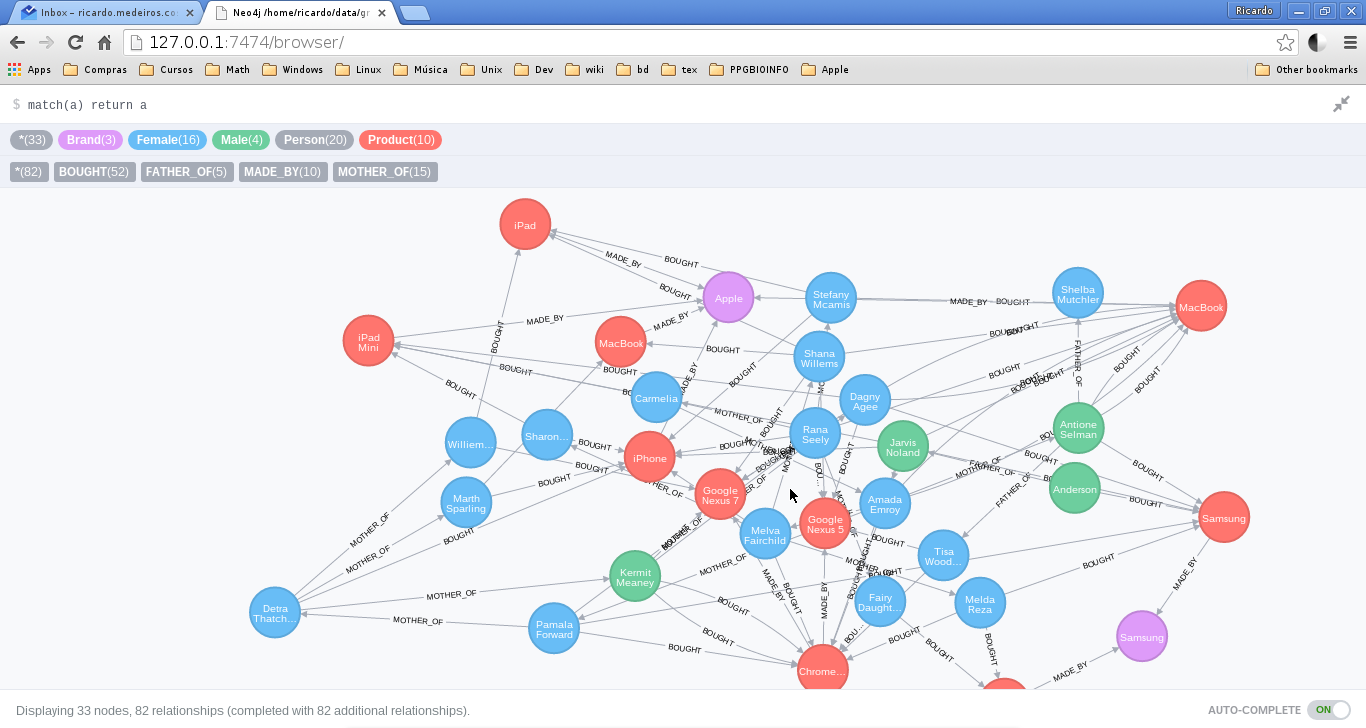
\includegraphics[width=1\textwidth]{1}
  \caption[1 - Banco de dados criado]{\textbf{Banco de dados criado}}
\end{figure} 

O banco criado possui 33 nós e 82 relações.

\section{Recomendações baseada em compras de produtos}
A lógica para essa consulta foi a seguinte: Relaciona com essa pessoa, produtos comprados por outras pessoas que compraram produtos iguais ao que a pessoa comprou. No entanto, são relacionados apenas produtos que a pessoa não comprou. O código da consulta \emph{Cypher} torna mais claro esse conceito. 

\begin{lstlisting}[frame=single]
match (person:Person)-[:BOUGHT]->(product:Product)
 <-[:BOUGHT]-(anotherPerson:Person)
  -[:BOUGHT]->(anotherProduct:Product)
where not (person)-[:BOUGHT]->(anotherProduct)
return person.name, collect(distinct anotherProduct.name)
order by person.name
\end{lstlisting}

O resultado: 
\begin{figure}[H]
  \centering
  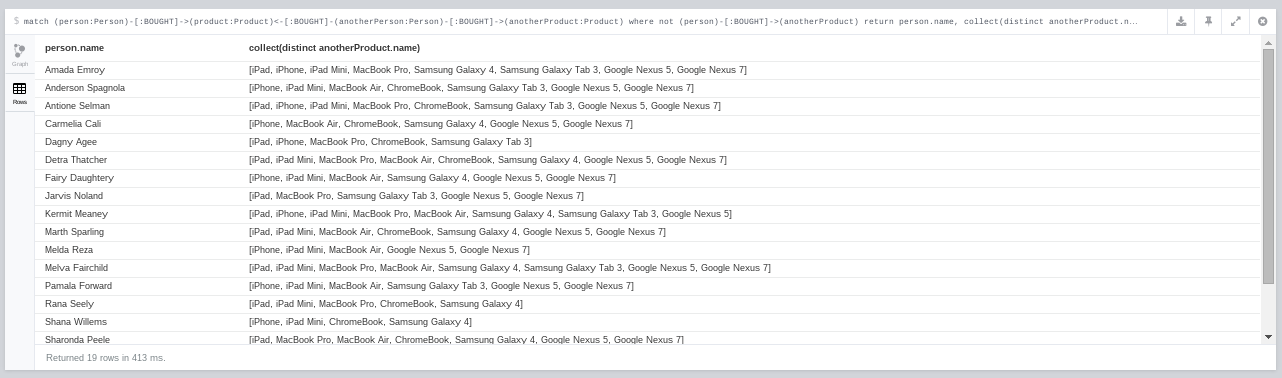
\includegraphics[width=1\textwidth]{2}
  \caption[2 - Recomendações baseadas em compra de produtos]{\textbf{Recomendações baseadas em compra de produtos}}
\end{figure} 

\section{Recomendações baseadas em lealdade à marca}
Para essa consulta, foi realizada uma consulta \emph{Cypher} que combina os nós pessoas que possuem compras de um produto de determinada marca e a partir desse relacionamento são relacionados outros produtos desta mesma marca. Assim como na consulta anterior, serão mostrados apenas os produtos que a pessoa não tenha comprado. A consulta: 

\begin{lstlisting}[frame=single]
match(person:Person)-[:BOUGHT]->(product:Product)-[:MADE_BY]->
(itsBrand:Brand)<-[:MADE_BY]-(recommendedProduct:Product)
where not (person)-[:BOUGHT]->(recommendedProduct)
return person.name, collect(distinct recommendedProduct.name)
order by person.name
\end{lstlisting} 

O resultado: 
\begin{figure}[H]
  \centering
  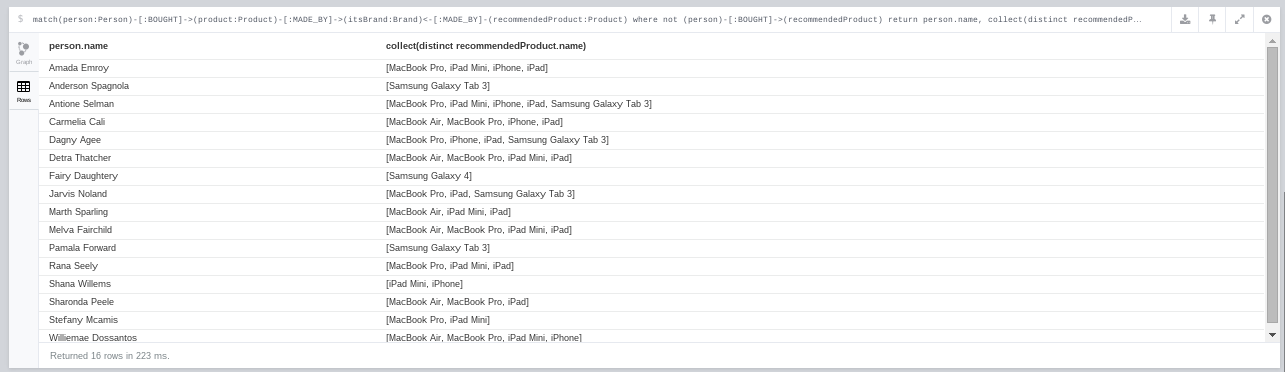
\includegraphics[width=1\textwidth]{3}
  \caption[3 - Recomendações baseadas em lealdade à marca]{\textbf{Recomendações baseadas em lealdade à marca}}
\end{figure}

\section{Recomendações baseadas em laçoes familiares}
Neste exercício foi necessário uma abordagem peculiar. Como não havia rótulo ou nenhuma propriedade \textbf{PAIS}, foi preciso verificar os filhos de um nó com relação \emph{ :FATHER\_OF} (pai de) ou\emph{ :MOTHER\_OF} (mãe de), pois de acordo com os dados persistidos no banco de dados, há irmãos apenas por parte de pai ou de mãe. A consulta: 

\begin{lstlisting}[frame=single]
match (brotherOrSister:Person)<-[:FATHER_OF|:MOTHER_OF]
-(parent:Person)-[:FATHER_OF|:MOTHER_OF]->
(person:Person)-[:BOUGHT]->(recommendedProduct:Product)
where not (brotherOrSister)-[:BOUGHT]->(recommendedProduct)
return brotherOrSister.name, collect(recommendedProduct.name)
order by brotherOrSister.name
\end{lstlisting}

O resultado:
\begin{figure}[H]
  \centering
  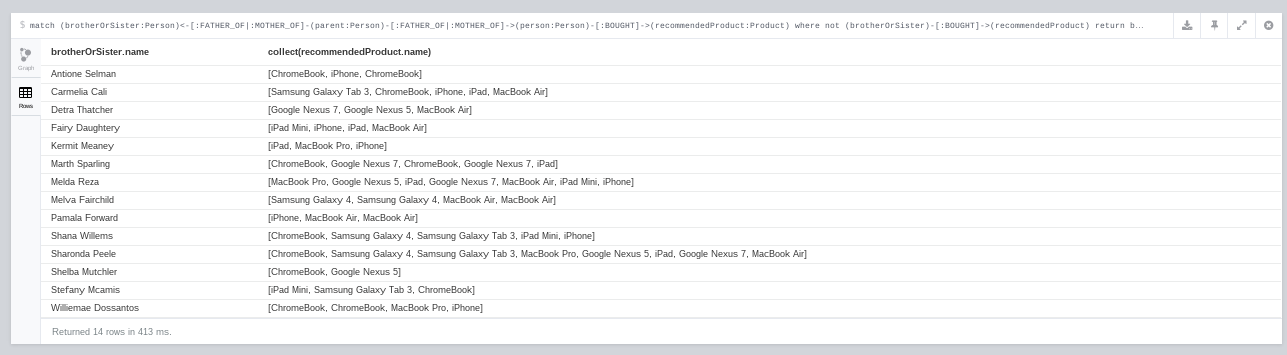
\includegraphics[width=1\textwidth]{4}
  \caption[4 - Recomendações baseadas em laçoes familiares]{\textbf{Recomendações baseadas em laçoes familiares}}
\end{figure} 

\end{document}
